\documentclass{amsart}
\usepackage{amssymb}
\usepackage{algorithmic}
\usepackage{comment}

\newtheorem{theorem}{Theorem}[section]
\newtheorem{lemma}[theorem]{Lemma}
\newtheorem{proposition}[theorem]{Proposition}
\newtheorem{corollary}[theorem]{Corollary}
\newtheorem{question}[theorem]{Question}\newtheorem{conjecture}[theorem]{Conjecture}

\theoremstyle{definition}
\newtheorem{definition}[theorem]{Definition}
\newtheorem{example}[theorem]{Example}
\newtheorem{problem}[theorem]{Problem}
\newtheorem{xca}[theorem]{Exercise}
\newtheorem{algorithm}[theorem]{Algorithm}

\theoremstyle{remark}
\newtheorem{remark}[theorem]{Remark}
\newtheorem{criterion}[theorem]{Criterion}

\numberwithin{equation}{section}

\newcommand{\B}[1]{\mathbb #1}
\newcommand{\C}[1]{\mathcal #1}
\newcommand{\F}[1]{\mathfrak #1}
\newcommand{\RM}[1]{\mathrm #1}
\newcommand{\SF}[1]{\mathsf #1}
\newcommand{\BF}[1]{\mathbf #1}

\newcommand{\alg}[1]{\operatorname{#1}}
\newcommand{\ideal}[1]{\langle #1 \rangle}
\newcommand{\norm}[1]{\| #1 \|_1}
%\newcommand{\dfrac}{\genfrac{}{}{}0}
%\newcommand{\tfrac}{\genfrac{}{}{}1}

\DeclareMathOperator{\SL}{SL}
\DeclareMathOperator{\GL}{GL}
\DeclareMathOperator{\SU}{SU}
\DeclareMathOperator{\Id}{Id}
\DeclareMathOperator{\poly}{poly}
\DeclareMathOperator{\initial}{in}
\DeclareMathOperator{\NF}{NF}
\DeclareMathOperator{\lcm}{lcm}
\DeclareMathOperator{\im}{im}
\newcommand{\dist}{d}
\newcommand{\actson}{\curvearrowright}
\newcommand{\cover}{\widetilde}
\newcommand{\closure}{\overline}
\newcommand{\Inc}{\operatorname{Inc}(\B N)}
\newcommand{\SymN}{\F S_\infty}
\newcommand{\Sn}{\tilde{\F S}_n}
\newcommand{\Snp}{\tilde{\F S}_{n'}}
\newcommand{\Sinf}{\F S_{\infty}^r}
\newcommand{\lleq}{\preceq}
\newcommand{\ggeq}{\succeq}
\newcommand{\llleq}{\sqsubseteq}
\newcommand{\gggeq}{\sqsupseteq}
\newcommand{\ZS}{\B Z^{\C S}}
\newcommand{\ZT}{\B Z^{\C T}}
\newcommand{\ZSn}{\B Z^{\C S_n}}
\newcommand{\ZTn}{\B Z^{\C T_n}}
\newcommand{\ZSone}{\B Z^{\C S_{(1,\ldots,1)}}}
\newcommand{\ZSC}{\ZS_{\mathbf{sc}}}
\newcommand{\Lin}{\mathrm{Lin}}
\newcommand{\mon}{M}
\newcommand{\Sym}{\F S_\infty}
\newcommand{\LT}{\initial_{\leq}}
\newcommand{\LTp}{\initial_{\leq'}}
\newcommand{\LC}{\operatorname{LC}}
\newcommand{\LM}{\operatorname{LM}}
\newcommand{\mm}{\C M}
\newcommand{\degtot}{\operatorname{deg}_{tot}}

\newcommand{\GB}{{Gr\"obner basis}}
\newcommand{\GBs}{{Gr\"obner bases}}

\begin{document} \title{Equivariant Gr\"obner bases}

 %   Information for first author 
\author{Christopher J. Hillar}
\address{Redwood Center for Theoretical Neuroscience, University of California, Berkeley}
\email{chillar@msri.org}

\author{Robert Krone}
\address{Georgia Tech University, Atlanta, GA}
\email{krone@math.gatech.edu}

\author{Anton Leykin}
\address{Georgia Tech University, Atlanta, GA}
\email{anton.leykin@gmail.com}

%\thanks{The work of the first author is supported under a National Science Foundation Graduate Research Fellowship.} 

\subjclass{13E05, 13E15, 20B30, 06A07}%

% \keywords{Invariant ideal, well-quasi-ordering, symmetric group, Gr\"obner basis, generating sets}


% \keywords{}


% ----------------------------------------------------------------
\begin{abstract}
The concept of an equivariant \GB\ in infinite dimensional polynomial rings enables symbolic computation with ideals finitely generated up to symmetry. We survey the existing approaches to computing equivariant \GBs and provide a new algorithm that incorporates the signature-based ideas that may reduce computational costs.
\end{abstract} 

\maketitle 
\tableofcontents
\section{Introduction}
 
\subsection{Basic definitions}

(Parts of preliminaries can go here).

\subsection{History}

(Early years: Cohen?)

(Rediscovery: Aschenbrenner-Hillar)

(Applications: Draisma, japanese statisticians?)

(Toric ideals: DEKL, etc.)

(Hilbert functions???: Nagel-Roemer)

(Gr\"obner categories: Sam-Snowden)

\subsection{Structure of the paper}

\section{Preliminaries}
Let $R$ be a commutative $K$-algebra equipped with a left action of monoid $\Pi$ (a $\Pi$-algebra structure).  We mainly consider the case where $R$ has the structure of a monoid algebra, that is for some abelian monoid $\mon$, the elements of $R$ consist of formal sums of elements of $\mon$ with coefficients in $K$.  An example of such a monoid algebra is polynomial ring $R = K[X]$ with variables from the set $X$.  In this case $\mon$ is the free abelian monoid generated by $X$, which we will denote by $[X]$.  To make our notation consistent with the polynomial case, we will denote the monoid algebra of $\mon$ over $K$ by $K\mon$ even though this is not standard (often it is written as $K[\mon]$ but this creates ambiguity with polynomial rings).  We will also generally refer to elements of $\mon$ as ``monomials'' in analogy to the polynomial case.  Additionally we will assume that $\Pi$ acts on monoid algebra $R$ through a $\Pi$-action on $\mon$ by monoid homomorphisms.

Our particular focus in this paper is when $\Pi$ is $\SymN$ or certain related monoids.  For our purposes $\SymN$ will be defined as the group of all finite permutations of $\B N$, meaning permutations that fix all but a finite number of elements.

\begin{example}
 Let $R = K[x_1,x_2,x_3,\ldots]$ with $\SymN$ acting on $R$ by permuting the variables, so that $\sigma x_i = x_{\sigma(i)}$.
\end{example}

\begin{definition}
 An ideal $I \subseteq R$ is a {\em $\Pi$-invariant ideal} if $\sigma I \subseteq I$ for all $\sigma \in \Pi$.
\end{definition}

The ring $R$ is both an $R$-algebra and a $\Pi$-algebra, and there is a ring $R*\Pi$ which captures both of these actions, and which will be referred to as the {\em twisted monoid ring} of $\Pi$ with coefficients in $R$.  The elements of $R*\Pi$ are of the form $\sum_{\sigma \in \Pi} f_{\sigma}\cdot \sigma$ with each $f_\sigma \in R$ and only a finite number non-zero.  The additive structure is the same as the usual monoid ring, but multiplication is ``twisted'' in that
 \[ (f\cdot \sigma)(g \cdot \tau) = f\sigma(g) \cdot \sigma\tau \]
where $\sigma(g)$ denotes the element of $R$ obtained by acting on $g$ by $\sigma$.

$R$ is a $R*\Pi$-module, and the definition of $\Pi$-invariant ideals can be restated as $R*\Pi$-submodules of $R$.

When $R = K\mon$ with $\Pi$ acting on $\mon$, then we can define monoid $\mon *\Pi$ whose elements are pairs in $\mon \times \Pi$ with monoid operation
 \[ (m, \sigma)(n, \tau) = (m\sigma(n), \sigma\tau). \]
There is a left action of $\mon*\Pi$ on $\mon$ and the elements of $\mon *\Pi$ are the ``monomials'' of $R*\Pi$.

\begin{definition}
 A $\Pi$-invariant ideal $I \subseteq R$ is {\em $\Pi$-finitely generated} if there is a finite set $F \subseteq I$ such that the $\Pi$-orbits of the elements of $F$ generate $I$.  Ring $R$ is called {\em $\Pi$-Noetherian} if every $\Pi$-invariant ideal in $R$ is $\Pi$-finitely generated.
\end{definition}
If a $\Pi$-invariant ideal $I$ is generated by the $\Pi$-orbits of a set $F$, we will write
 \[ I = \ideal{F}_{\Pi}. \]
Such a set $F$ generates $I$ as an $R*\Pi$-module.

We can also say that monoid $\mon$ with $\Pi$-action is $\Pi$-finitely generated if it generated by the $\Pi$-orbits of a finite number of elements.  Then $R = K\mon$ is $\Pi$-finitely generated as a $K$-algebra.

\begin{example}
 Continuing the above example of $R = K[x_1,x_2,x_3,\ldots]$ with $\SymN$ action, the ideal $\F m = \ideal{x_1,x_2,x_3,\ldots}$ is a $\SymN$-invariant ideal.  Moreover, it is $\SymN$-finitely generated because $\F m = \ideal{x_1}_{\SymN}$.  Also $R$ is a $\SymN$-finitely generated $K$-algebra with generator $x_1$.
\end{example}
 

\begin{definition}
 Let $R$ be a $\SymN$-algebra.  For $f \in R$, the {\em width} of $f$ is the smallest integer $n$ such that for every $\sigma \in \SymN$ that fixes $\{1,\ldots,n\}$, $\sigma$ also fixes $f$.  The width of $f$ is denoted $w(f)$.  If no such integer $n$ exists, then $w(f) = \infty$.  For a set $F \subseteq R$, its width is $w(F) := \max_{f \in F}\{w(f)\}$.
\end{definition}
If every element of $R$ has finite width, we will say that $R$ satisfies the {\em finite width condition}.  This is primarily the situation we want to address in this paper, and so we will assume from here forward that all rings with $\Sym$-action satisfy the finite width condition unless stated otherwise.  For a $\SymN$-invariant ideal $I \subseteq R$ and an integer $n$ we can define the $n$th truncation of $I$ as
 \[ I_n := \{ f \in I \mid w(f) \leq n \}. \]
The set $I_n$ is naturally a $\F S_n$-invariant ideal of $R_n$.  If $R$ satisfies the finite width condition, then $I$ is the union of all of its truncations.  If moreover $I$ is $\SymN$-finitely generated, then there is sufficiently large $n \in \B N$ such that $I = \ideal{I_n}_{\SymN}$.

The definition of width also applies to $\Pi = \Inc$, the monoid of strictly increasing functions, which is introduced below.
 
\begin{definition}
 Given $R = K\mon$ with $\Pi$ acting on $\mon$, there is a natural partial order $|_\Pi$ on $\mon$ called the {\em $\Pi$-divisibility partial order} defined by $a |_\Pi b$ if there exists $\sigma \in \Pi$ such that $\sigma a$ divides $b$.  Equivalently $a |_\Pi b$ if $b \in \ideal{a}_\Pi$.
\end{definition}

Recall that a monomial order on $R = K\mon$ is a total order $\leq$ on $\mon$ that is a well-order, and that respects multiplication, meaning if $a \leq b$ then $ac \leq bc$ for all $c \in \mon$.

\begin{definition}
 A monomial order $\leq$ on $R = K\mon$ {\em respects $\Pi$} if whenever $a \leq b$ then $\sigma a \leq \sigma b$ for all $\sigma \in \Pi$.
\end{definition}

Therefore order $\leq$ is a $\Pi$-respecting monomial order on $R$ if $\leq$ is a total well-order on $M$ that respects the action of $\mon*\Pi$.
Now we have the tools to describe the $\Pi$-equivariant version of Gr\"obner bases.
\begin{definition}
 Let $R = K\mon$ be a monoid ring with $\Pi$ action on $\mon$, and let $\leq$ be a $\Pi$ respecting monomial order.  Given a $\Pi$-invariant ideal $I \subseteq R$, a {\em $\Pi$-equivariant Gr\"obner basis} of $I$ is a set $G \subseteq I$ such that the $\Pi$ orbits of $G$ form a Gr\"obner basis of $I$,
 \[ \ideal{\LT \Pi G} = \LT I. \]
\end{definition}
We require $\leq$ to be a $\Pi$ respecting order because it is equivalent to the condition that
\[ \LT \sigma f = \sigma \LT f \]
for all $f \in R$ and $\sigma \in \Pi$.  Therefore with such an order
 \[ \ideal{\LT G}_{\Pi} = \ideal{\LT \Pi G} = \LT I. \]
This also implies that $\LT I$ is a $\Pi$-invariant ideal.  Note that since the $\Pi$ orbits of $G$ are a Gr\"obner basis of $I$, we have $\ideal{G}_\Pi = I$.


\begin{proposition}[Remark 2.1 of \cite{Brouwer09e}]\label{prop:nogroup}
 Let $\Pi$ be a group which acts non-trivially on $\mon$.  Then $K\mon$ has no $\Pi$ respecting monomial orders.
\end{proposition}
\begin{proof}
 Suppose that $\leq$ is a $\Pi$ respecting order and choose $\sigma \in \Pi$ and $m \in \mon$ such that $m \neq \sigma m$.  If $m > \sigma m$ then $\sigma^n m > \sigma^{n+1} m$ for all $n$ so
  \[ m > \sigma m > \sigma^2 m > \cdots \]
 is an infinite descending chain of monomials, contradicting the fact that $\leq$ is a well-order.  If $m < \sigma m$ then $m > \sigma^{-1} m > \sigma^{-2} m > \cdots$ is an infinite descending chain.
\end{proof}

In particular this means that $R$ with non-trivial $\Sym$ action has no $\Sym$ respecting monomial orders.  To deal with this problem, a related monoid is introduced to replace $\Sym$ which allows for monomial orders but is somehow large enough compared to $\Sym$ not to break properties like finite generation.

Define the {\em monoid of strictly increasing functions} as
\[ \Inc := \{ \rho:\B N \to \B N \mid \text{ for all } a < b, \rho(a) < \rho(b) \}. \]
For any $\Sym$-algebra $R$ with the finite width property, there is a natural action of $\Inc$ on $R$ as follows.  Fixing $f \in R$, for any $\sigma \in \Sym$ the value of $\sigma f$ depends only on the restriction $\sigma|_{[w(f)]}$ considering $\sigma$ as a function $\B N \to \B N$.  For any $\rho \in \Inc$ there exists $\sigma \in \Sym$ such that $\sigma|_{[w(f)]} = \rho|_{[w(f)]}$ and define $\rho f = \sigma f$.  It can be checked that this gives a well-defined action of $\Inc$ on $R$.

It immediately follows from the definition of the action that $\Inc f \subseteq \Sym f$.  Despite the fact that $\Inc$ is not a submonoid of $\Sym$, it behaves like one in terms of its action on $R$.  An injective map $\sigma|_{[w(f)]}: [w(f)] \to \B N$ can always be factored into $\rho' \circ \tau$ with $\tau \in \F S_{w(f)}$ and $\rho':[w(f)] \to \B N$ a strictly increasing function.  The map $\rho'$ can be extended to some $\rho \in \Inc$, and then $\sigma f = \rho (\tau f)$.  Thus
 \[ \Sym f = \bigcup_{\tau \in \F S_{w(f)}} \Inc(\tau f). \]
This fact that the $\Sym$-orbit of any $f$ is a finite union of $\Inc$-orbits implies the following statements.

\begin{proposition}
 Let $R$ be a $\Sym$-algebra satisfying the finite width condition, and let $I\subseteq R$ be a $\Sym$-invariant ideal.
 \begin{itemize}
  \item $I$ is $\Inc$-invariant.
  \item $I$ is $\Sym$-finitely generated if and only if $I$ is $\Inc$-finitely generated.
  \item If $R$ is $\Inc$-Noetherian then $R$ is $\Sym$-Noetherian.
 \end{itemize}
\end{proposition}

When computing Gr\"obner bases of $\Sym$-invariant ideals we will work with the $\Inc$ action instead.  If $G$ is an $\Inc$-equivariant Gr\"obner basis for $\Sym$-invariant ideal $I$, then the $\Sym$-orbits of $G$ also form a Gr\"obner basis of $I$.  Generally the rings we are interested in will have $\Inc$ respecting monomial orders.

\begin{example}
 Let $R = K[x_1,x_2,\ldots]$ with $\Inc$-action defined by $\rho \cdot x_i = x_{\rho(i)}$.  The lexicographic order $\leq$ on the monomials of $R$ with $x_1 < x_2 < x_3 < \cdots$ is a $\Inc$ respecting monomial order.  This is the only possible lexicographic order on $R$ that respects $\Inc$.  There are also a graded lexicographic and a graded reverse lexicographic order on $R$ that respect $\Inc$.  There is no $\Inc$ respecting monomial order on $R$ that is defined by a single weight vector in $\B R^{\B N}$.
\end{example}

It is an open question to characterize all possible $\Inc$ respecting monomial orders on a given ring $K\mon$ with $\Inc$ action.  We can make the following statement about such orders.

\begin{proposition}
 If $\leq$ is a $\Pi$ respecting monomial order on $K\mon$, then $\leq$ refines the $\Pi$-divisibility quasi-order $|_\Pi$.
\end{proposition}
\begin{proof}
 Suppose $a$ and $b$ are monomials with $a |_\Pi b$, so there is some pair $\sigma \in \Pi$, $c \in \mon$ such that $c\sigma a = b$.  From the proof of Proposition \ref{prop:nogroup} we see that $a \leq \sigma a$.  Since $1 \leq c$ and $\leq$ respects multiplication, $\sigma a \leq c\sigma a = b$.
\end{proof}

A implication of this proposition is that if $K\mon$ has a $\Pi$ respecting monomial order then the $\Pi$-divisibility quasi-order must be a partial order, meaning it has the anti-symmetry property: if $a \geq b$ and $a \leq b$ then $a = b$.  If anti-symmetry fails for $|_\Pi$, it will also fail for any refinement.

If $R$ is $\Pi$-Noetherian with a $\Pi$ respecting monomial order, then any $\Pi$-invariant ideal $I \subseteq R$ will have a finite $\Pi$-equivariant Gr\"obner basis.  This follows from the fact that $\LT I$ is $\Pi$-finitely generated.  We recount two previous results that give examples of $\Inc$-Noetherian rings, and will be directly relevant to the results of this paper.

\begin{theorem}[Theorem 1.1 of \cite{hillar2012finite}]\label{thm:HS}
 Let $X = \{x_{ij} \mid i \in [k], j \in \B N\}$, and let $\Sym$ act on $[X]$ by permuting the second index, $\sigma x_{ij} = x_{i\sigma(j)}$ for $\sigma \in \Sym$.  Then $K[X]$ is $\Inc$-Noetherian.
\end{theorem}

\begin{theorem}[Theorem 1.1 of \cite{draisma2013noetherianity}]\label{thm:DEKL}
 Let $K[Y]$ be a $\Sym$-algebra with $\Sym$ action on variable set $Y$.  Suppose $Y$ has a finite number of $\Sym$-orbits, and $K[Y]$ satisfies the finite width condition.  For $K[X]$ defined as in Theorem \ref{thm:HS}, let $\phi$ be a monomial map
  \[ \phi: K[Y] \to K[X]. \]
 Then
 \begin{itemize}
  \item $\ker \phi$ is $\Inc$-finitely generated,
  \item $\im \phi$ is $\Inc$-Noetherian.
 \end{itemize}
\end{theorem}

The conditions on ring $K[Y]$ in Theorem \ref{thm:DEKL} are quite general and Hillar and Sullivant \cite{hillar2012finite} prove that such rings are generally not $\Sym$-Noetherian.  They give the example of $K[Y]$ where $Y = \{y_{ij} \mid i, j \in \B N\}$ with $\sigma y_{ij} = y_{\sigma(i)\sigma(j)}$ for $\sigma \in \Sym$ and prove that Noetherianity fails.

When $R$ is not $\Pi$-Noetherian, we do not know in general if a $\Pi$-finitely generated ideal $I\subseteq R$ has a finite $\Pi$-equivariant Gr\"obner basis, or if so, for which monomial orders.  However we will prove in Section \ref{sec:egbtoric} that the $\Sym$-invariant toric ideal $\ker \phi$ as in Theorem \ref{thm:DEKL} does have finite $\Inc$-equivariant Gr\"obner bases for specifically chosen monomial orders.  This will allow an algorithm to compute such a Gr\"obner basis of $\ker \phi$, given the map $\phi$.

\section{Equivariant Buchberger algorithm}
\subsection{Description of the algorithm}
First proposed in \cite{aschenbrenner2007finite} and formalized in \cite{Brouwer09e}, Buchberger's algorithm can be adapted to the equivariant setting in a straightforward way.

Let $R = K\mon$ with $\Pi$ acting on $\mon$, and let $\leq$ be a $\Pi$ respecting monomial order.  For $f,g \in R$ say that $g$ {\em $\Pi$-reduces} $f$ if $\LT g |_{\Pi} \LT f$ and the reduction is $f - \frac{\LC(f)}{\LC(g)}mg$ where $m \in \mon *\Pi$ such that $\LT f = m\LT g$ (and $\LC(f)$ denotes the lead coefficient of $f$).  For $G \subseteq R$, a {\em $\Pi$-normal form} of $f$ with respect to $G$ denoted $\NF_{\Pi G}(f)$ is the result of repeated $\Pi$-reductions of $f$ by elements of $G$ until no more reductions are possible.  Equivalently $\NF_{\Pi G}(f)$ is a normal form of $f$ with respect to $\Pi G$.

The equivariant Buchberger algorithm is described below, which departs from the conventional Buchberger algorithm only at the step of adding new S-pairs to the list $S$.  This departure is described after, along with a definition of $O_{f,g}$ and the ``finite S-pair condition.''

\begin{algorithm}[Brouwer--Draisma \cite{Brouwer09e}]\label{alg:Buchberger}
$G = \alg{Buchberger}(F)$
\begin{algorithmic}[1]
\REQUIRE $F$ is a finite set of elements in $R = K\mon$ with $\Pi$ acting on $\mon$ and satisfying the finite S-pair condition.
\ENSURE $G$ is $\Pi$-equivariant Gr\"obner basis of $\ideal{F}_{\Pi}$.

\smallskip \hrule \smallskip

\STATE $G\gets F$
\STATE $S\gets \bigcup_{f,g\in G} O_{f,g}$
\WHILE{$S\neq\emptyset$}
	\STATE pick $(h_1,h_2) \in S$
	\STATE $S\gets S\setminus\{(h_1,h_2)\}$ 
	\STATE $h \gets \NF_{\Pi G}(h_1 - \frac{\LC(h_1)}{\LC(h_2)}h_2)$
  	\IF{$h \neq 0$}
		\STATE $G\gets G\cup \{h\}$
		\STATE $S\gets S\cup \left(\bigcup_{g\in G}O_{g,h}\right)$
	\ENDIF
\ENDWHILE
\smallskip \hrule \smallskip
\end{algorithmic}
\end{algorithm}

Given $f,g \in R$ define
 \[ \C S_{f,g} := \{(m_1f,m_2g) \mid m_1,m_2 \in \mon * \Pi \text{ such that } \LT m_1f = \LT m_2g\}. \]
This set is closed under the diagonal action of $\mon *\Pi$ making $\C S_{f,g}$ a $\mon *\Pi$-module.  A set $G \subseteq R$ satisfies the {\em equivariant Buchberger criterion} if for all $(h_1,h_2) \in \bigcup_{f,g\in G} \C S_{f,g}$,
 \[ \NF_{\Pi G}(h_1 - \tfrac{\LC(h_1)}{\LC(h_2)}h_2) = 0. \]
The set $G$ is a $\Pi$-equivariant Gr\"obner basis of $\ideal{G}_{\Pi}$ if and only if it satisfies the equivariant Buchberger criterion.  The proof of this fact follows by applying the usual Buchberger criterion to the set $\Pi G$ (see Theorem 2.5 of \cite{Brouwer09e}).

For each pair $f,g \in G$, we need not check the criterion on every pair in $\C S_{f,g}$ which is an infinite set.  It is instead sufficient to check on a $\mon * \Pi$ generating set of $\C S_{f,g}$, which we denote $O_{f,g}$.  Still in general it may be that no finite generating set of $\C S_{f,g}$ exists, in which case we cannot apply the algorithm in finite time.

\begin{definition}
 A $\Pi$-algebra $R = K\mon$ has the {\em finite S-pair condition} if for any $f,g \in R$, the set $\C S_{f,g}$ is finitely generated as a $\mon * \Pi$-module.  In \cite{Brouwer09e} this condition is referred to as ``EGB4.''
\end{definition}

When $\Pi$ is trivial and $R$ is a polynomial ring (the setting of the conventional Buchberger algorithm), $\C S_{f,g}$ is generated by a single pair $(m_1 f,\; m_2 g)$ where $m_1 = \lcm(\LT f, \LT g)/\LT(f)$ and $m_2 = \lcm(\LT f, \LT g)/\LT(g)$.  This generator is typically referred to as the ``S-pair'' of $f,g$.  Therefore $R$ in this case satisfies the finite S-pair condition, and the equivariant Buchberger algorithm specializes to the conventional Buchberger algorithm.

\begin{proposition}
 If $R$ is a polynomial ring $R = K[Y]$ with $\Inc$-action on $[Y]$ satisfying the finite width condition, then $R$ has the finite S-pair condition.
\end{proposition}
\begin{proof}
 Fix $f,g \in R$.
 Since $R$ is a polynomial ring, for fixed $\sigma_1,\sigma_2 \in \Inc$, all elements of $\C S_{f,g}$ of the form $(m_1\sigma_1 f, m_2\sigma_2 g)$ with $m_1,m_2 \in \mon$ are monomial multiplies of the usual S-pair of $\sigma_1 f, \sigma_2 g$,
  \[ \left(\frac{m}{\LT \sigma_1 f} \sigma_1 f,\; \frac{m}{\LT \sigma_2 g} \sigma_2 g\right) \]
 where $m = \lcm(\LT \sigma_1 f,\LT \sigma_2 g)$.

 Any $f,g \in R$ have finite width so $\sigma_1 f$ depends only on $\sigma_1|_{[w(f)]}$, and similarly for $\sigma_2 g$.  In fact we can always factor the pair as
  \[ (\sigma_1 f, \sigma_2 g) = \tau(\rho_1 f, \rho_2 g) \]
 for some $\tau \in \Inc$, while $\rho_1:[w(f)] \to [w(f) + w(g)]$ and $\rho_2:[w(g)] \to [w(f) + w(g)]$ are strictly increasing functions.  Here $\rho_1$ and $\rho_2$ are chosen to ``interlace'' the variables of $f$ and $g$ in the same way as $\sigma_1,\sigma_2$.  (To consider $\rho_1,\rho_2$ as elements of $\Inc$, take any choice of extensions to maps on $\B N$.)
 
 Then $\C S_{f,g}$ is generated by the finite set of pairs of the form
  \[ \left(\frac{m}{\LT \rho_1 f} \rho_1 f,\; \frac{m}{\LT \rho_2 g} \rho_2 g\right) \]
 with $\rho_1:[w(f)] \to [w(f) + w(g)]$ and $\rho_2:[w(g)] \to [w(f) + w(g)]$ where $m = \lcm(\LT \rho_1 f,\LT \rho_2 g)$.
\end{proof}
\begin{comment}
\begin{figure}[ht]\label{fig:interlace}
  \centering
  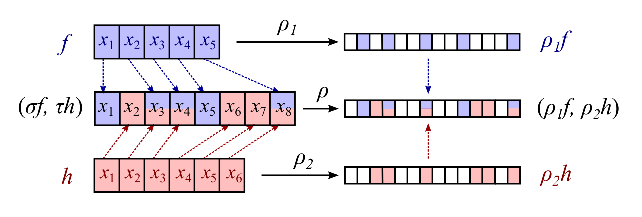
\includegraphics[width=.7\columnwidth]{incmap.ps}
  \caption{A pair of}
\end{figure}
\end{comment}

We note that Algorithm \ref{alg:Buchberger} is guaranteed to terminate when $R$ is $\Pi$-Noetherian.  Let $G_0,G_1,\ldots$ be the value of $G$ at each step.  The initial ideals of these sets form a strictly increasing chain of $\Pi$-invariant monomial ideals
 \[ \ideal{\LT G_0}_\Pi \subsetneq \ideal{\LT G_1}_\Pi \subsetneq \cdots \]
which must terminate.  However, without Noetherianity, we offer no termination guarantee of the algorithm as stated above, even when a finite equivariant Gr\"obner basis for the ideal exists.  In the next section we give a modification of the algorithm which repairs this when $\Pi = \Inc$ and certain conditions on $R$ are met.

\subsection{Termination of $\Inc$-equivariant Buchberger}
Let $R = K\mon$ with $\Inc$ action on $\mon$, with $R$ satisfying the finite width and finite S-pair conditions, and with each truncation $R_n$ a Noetherian ring.  (These conditions are satisfied for example when $R = K[Y]$ where $Y$ consists of a finite number of orbits of variables, as in Theorem \ref{thm:DEKL}.)   Let $I \subseteq R$ be a $\Inc$-invariant ideal which is $\Inc$-generated by finite set $F$, and moreover has finite $\Inc$-equivariant Gr\"obner basis $G$.  Define the {\em generator truncation} of $I$ to be $\tilde{I}_{F,n} := \ideal{\Inc F \cap R_n} \cap R_n$.  Note that $\tilde{I}_{F,n} \subseteq I_n$ but in general equality does not hold.  For $f \in I$ define $w_F(f)$ to be the minimum value of $n$ for which $f \in \tilde{I}_{F,n}$.

The truncated EGB algorithm again takes finite generating set $F$ as its input.  For each successive $n \geq w(F)$, compute a set $G_n$ such that $\Inc G_n \cap R_n$ is a Gr\"obner basis for $\tilde{I}_{F,n}$.  Then check if $G_n$ is a $\Inc$-equivariant Gr\"obner basis of $I$ using the equivariant Buchberger criterion, and if so return $G_n$.

\begin{algorithm}\label{alg:truncBuch}
$G = \alg{TruncatedEGB}(F)$
\begin{algorithmic}[1]
\REQUIRE $F$ is a finite set of elements in $R = K\mon$ with $\Inc$ acting on $\mon$, $R$ satisfies the finite width and finite S-pair conditions, and each $R_n$ is Noetherian.
\ENSURE $G$ is a $\Inc$-equivariant Gr\"obner basis of $I := \ideal{F}_{\Inc}$.

\smallskip \hrule \smallskip

\STATE $G\gets F$
\STATE $n\gets w(F)$
\WHILE{$G$ not a $\Inc$-equivariant Gr\"obner basis of $I$}
	\STATE $G\gets$ Gr\"obner basis of $\tilde{I}_{F,n}$
	\STATE $n \gets n+1$
\ENDWHILE
\smallskip \hrule \smallskip
\end{algorithmic}
\end{algorithm}

\begin{proof}[proof of termination]
For each $n$, let $G_n$ denote the value of $G$ after that step.  Computing $G_n$ is a finite process since it takes place in $R_n$ which is Noetherian.  $G_n$ is a finite set and so it has a finite number of S-pairs to be checked.  Therefore testing whether $G_n$ is a $\Inc$-equivariant Gr\"obner basis is finite.

It remains to be proved that $G_n$ is a $\Inc$-equivariant Gr\"obner basis for some value of $n$.  If $H$ is a $\Inc$-equivariant Gr\"obner basis of $I$, for any $h \in H$ we have $h \in \tilde{I}_{F,n}$ for all $n \geq w_F(h)$, so $\LT(h) \in \LT(\tilde{I}_{F,n})$.  Therefore there is some element $g \in G_n$ with $\LT(g)|_{\Inc} \LT(h)$.  For $n = \max_{h\in H} w_F(h)$, the initial ideal $\ideal{\LT(G_n)}_{\Inc}$ contains $\ideal{\LT(H)}_{\Inc}$ and so $G_n$ is a $\Inc$-equivariant Gr\"obner basis of $I$.
\end{proof}

In practice, $G_n$ can be computed either using a traditional Gr\"obner basis algorithm on input $\Inc F \cap R_n$, or using an equivariant Buchberger algorithm on input $F$ with the following two caveats:
\begin{itemize}
 \item consider only S-pairs $(m_1f, m_2g)$ with $m_1f$ and $m_2g$ both having width $\leq n$,
 \item perform only reductions such that the outcome has width $\leq n$.
\end{itemize}
Moreover we do not need to restart the algorithm from scratch for each $n$.  Instead $G_{n-1} \cup F$ can be used as the input for the $n$th step instead of $F$.

Suppose $R$ has the form $K[Y]$ and each $R_n = K[Y_n]$ for some $Y_n \subseteq Y$.  If $\leq$ is a width order (a monomial order such that $w(a) < w(b)$ implies $a < b$), the second condition is satisfied automatically since reductions cannot increase the width.  Therefore the normal form of a given S-pair does not depend on $n$ and only needs to be computed once.  As a result we can use Algorithm \ref{alg:Buchberger}, queuing S-pairs by width so that the smallest width S-pairs are considered first.  The algorithm terminates once the queue is empty.  A separate check for whether $G_n$ is a $\Inc$-equivariant Gr\"obner basis for $I$ is not needed since this is equivalent to reducing all S-pairs in the queue.

\section{A signature-based approach}

Here we decribe our new approach to computing equiavriant \GBs\ utilizing the information stored in {\em signatures}. 

Signature-based algorithms for computing \GBs\ in the most common (finite-dimensional commutative) setting acquired popularity due to Faugere's F5 (see a short description in \S 4 of Chapter 10 of the new edition of Cox, Little, and O'Shea~\cite{Cox-Little-OShea:I-V-A}) and several other recent works (refs?).      
One of the most concise theoretical setups of a signature-based algorithm is given by Gao {\em et al.} in \cite{Gao-Volny-Wang:signature-GBs}.  

\subsection{Strong \GB}
(describe Gao's approach here)

\subsection{Translation to an equivariant setting}
Main point: the direct translation is impossible!

\bibliographystyle{plain}
\bibliography{egb}

\end{document}
% ----------------------------------------------------------------

